\section{Vibrational–Rotational Transitions of Diatomic Molecules}

\begin{figure}[]
 \begin{center}
	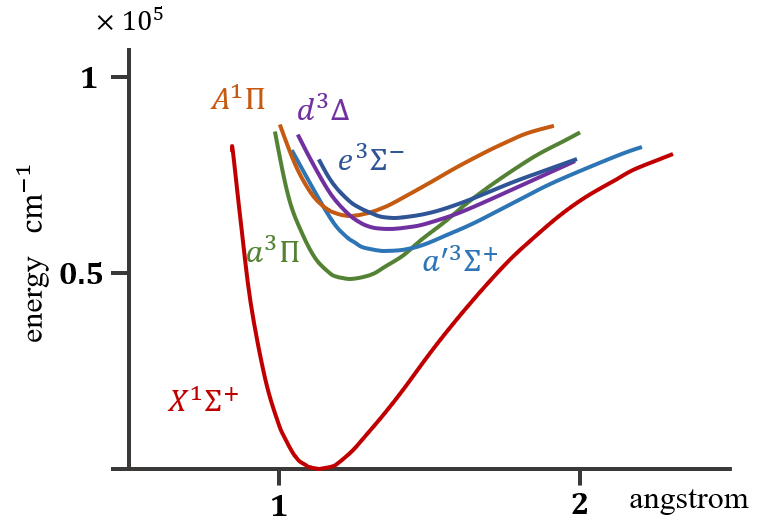
\includegraphics[width=1.0\linewidth]{fig/co_ele_state.png}
% 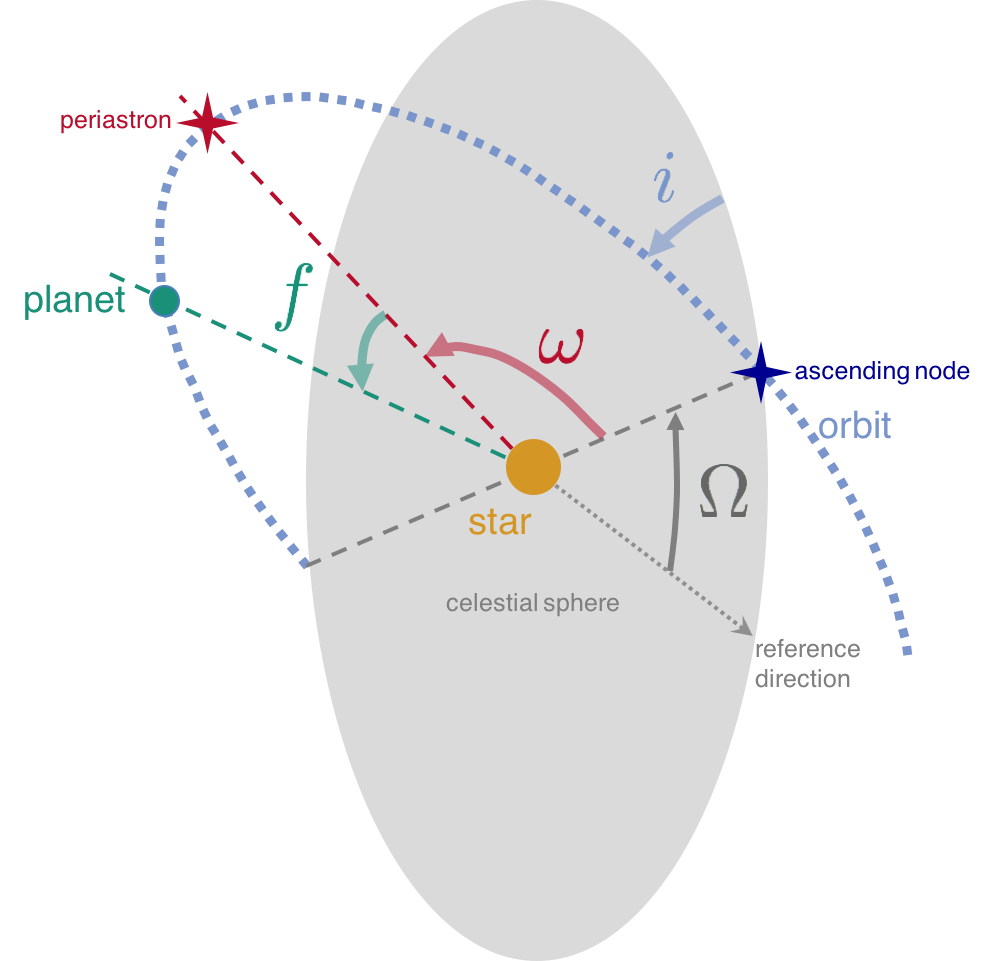
\includegraphics[bb=0 0 474 461,width=1.0\linewidth]{fig/orbele.png}
\end{center}
\caption{Electronic states of carbon monoxide. The horizontal axis is the internuclear distance (carbon–oxygen).}
\label{fig:co_ele_state}
\end{figure} 

In diatomic molecules, quantum-mechanical transitions arise from combinations of electronic, vibrational (nuclear), and rotational (nuclear) level transitions. For the electronic levels, because nuclear motion is much slower than electronic motion, one can solve the electronic wave equation with the internuclear distance $r$ fixed and obtain the corresponding electronic eigenenergies.

As $r$ is slowly varied, the ground-state electronic eigenenergy changes continuously with $r$. Figure~\ref{fig:co_ele_state} shows (a subset of) the electronic eigenenergies of carbon monoxide as a function of the internuclear distance $r$. In the context of molecular absorption in exoplanet atmospheres, it is generally safe to assume that the electronic state is the ground state ( in the case of CO, $\mathrm{X^1}\Sigma^+$)\footnote{Electronic transitions are occasionally considered as well.}. Thus, the ground-state electronic eigenenergy can be written as a function of $r$ as $V(r)$, and the two nuclei can be regarded as moving in the potential $V(r)$.

\begin{itembox}{{\it column} -- Labels of Electronic States $\,^\dagger$}
%\tiny
\footnotesize
For diatomic molecules, the magnitude $\Lambda$ of the projection of the total electronic orbital angular momentum onto the molecular axis ($Z$ axis), $L_z$, is conserved, and $\Lambda$ serves as a label for the electronic state. The spectroscopic symbols corresponding to each $\Lambda$ are summarized in Table~\ref{tab:spesymbol}. As in atoms, spin multiplicity exists for molecules. With total spin $S$ ($S=0,1/2,1,3/2,\cdots$), the multiplicity is $2S+1$, written to the upper left of $\Lambda$:
\begin{eqnarray}
    \,^{2S+1} \Lambda.
\end{eqnarray}
If the diatomic molecule consists of two identical atoms (homonuclear diatomic), the wavefunction under exchange of the two nuclei transforms as $\Psi \to \pm \Psi$. The symbol \emph{u} (ungerade) is appended as a subscript when the sign changes, and \emph{g} (gerade) when it does not. In addition, for $\Sigma$ states, the sign change under reflection through a plane containing the molecular axis is indicated by a superscript $\pm$. Altogether, an electronic state can be labeled, for example, as
\begin{eqnarray}
    \,^{2} \Sigma_u^+ .
\end{eqnarray}
Table~\ref{tab:elebase} lists the ground states of representative diatomic molecules. Among electronic states with the same spin multiplicity, one may also prepend capital letters X, B, C, D, $\cdots$ (including the ground state) in increasing energy order. For states with spin multiplicity different from that of the ground state, lowercase letters b, c, d, $\cdots$ are sometimes used in increasing energy order; e.g.,
$X\,^1 \Sigma_g^+$ (ground state), $B\,^1 \Sigma_u^+$, $C\,^1 \Sigma_u^+$, …, $a\,^3 \Sigma$, …
\end{itembox}

\begin{table}[]
    \centering
    \begin{tabular}{c|cccccc}
    \hline\hline
        $L$ & 0 & 1 & 2 & 3 & $\cdots$  \\
        \hline
          & S & P & D & F & $\cdots$  \\
          Degeneracy & 1 & 3 & 5 & 7 & (2$L$+1) \\
        \hline\hline
        $\Lambda$ & 0 & 1 & 2 & 3 & $\cdots$  \\
        \hline
        & $\Sigma$ & $\Pi$ & $\Delta$ & $\Phi$ & $\cdots$ \\
        Degeneracy & 1 & 2 & 2 & 2 &  
    \end{tabular}
    \caption{Correspondence between the electronic orbital angular momentum $L$ for atoms and the absolute value of the molecular-axis projection $L_z$ for diatomic molecules, $\Lambda$, and the spectroscopic symbols. For atoms the degeneracy is $2L+1$, whereas for molecules (except for $\Lambda=0$), the two projections $L_z=\pm \Lambda$ lead to twofold degeneracy.}
    \label{tab:spesymbol}
\end{table}

\begin{table}[]
    \centering
    \begin{tabular}{c|c}
    \hline\hline
    Molecule & Ground State\\
    \hline
        \ce{H2} & $\,^1 \Sigma_g^+$\\
        \ce{N2} & $\,^1 \Sigma_g^+$\\
        \ce{O2} & $\,^3 \Sigma_g^-$\\
        \ce{CO} &  $\,^1 \Sigma$\\
        \ce{CN} &  $\,^2 \Sigma$\\
        \ce{NO} &  $\,^2 \Pi$
    \end{tabular}
    \caption{Electronic ground states of representative diatomic molecules.}
    \label{tab:elebase}
\end{table}

Let us now consider the energy levels of a freely moving diatomic molecule, such as carbon monoxide (CO) in an atmosphere, which consists of two nuclei with different masses $m_1$ and $m_2$ and multiple electrons. Assuming the electrons remain in the ground state, the system can be treated as two nuclei moving in the potential $V(r)$, where $r$ is the internuclear distance. As illustrated in the ground state of Fig.~\ref{fig:co_ele_state}, $V(r)$ attains its minimum value (we define it by $V_e$) at $r=r_e \sim 1.2 \AA$, and the two nuclei undergo rotational motion and vibrational motion about the equilibrium distance $r_e$.

\begin{figure}[h]
\begin{center}
%  \includegraphics[width=70mm]{fig_left.PNG}
  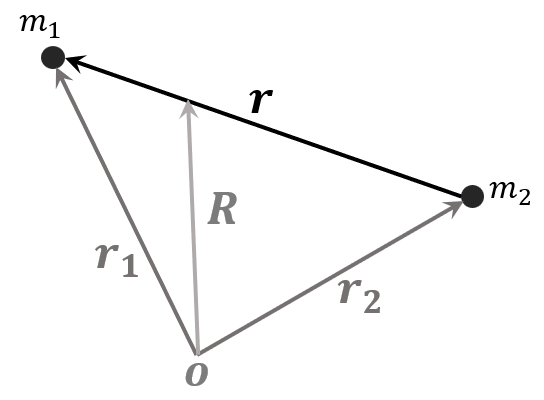
\includegraphics[width=\linewidth]{fig/fig_right.PNG}
\end{center}
\vspace*{-5mm}
\caption{Coordinates of the nuclei in a diatomic molecule.}
\label{fig:phys2_fig1}
\end{figure}

Assuming that $V(r)$ is known, we focus on the nuclear wave equation.  
With nuclear coordinates taken as in Fig.~\ref{fig:phys2_fig1}, the nuclear wave equation can be written as
\begin{align}
\label{eq:phys2_shro}
&\left( - \frac{\hbar^2}{2 m_1} \nabla_{1}^2  - \frac{\hbar^2}{2 m_2} \nabla_{2}^2 + V(r) \right) \psi(\boldsymbol{r}_1, \boldsymbol{r}_2) \nonumber \\
&= E \psi(\boldsymbol{r}_1, \boldsymbol{r}_2),
\end{align}
where $\boldsymbol{r}_1$ and $\boldsymbol{r}_2$ are the position vectors of nuclei 1 and 2, respectively, and their separation is $r = |\boldsymbol{r}_1 - \boldsymbol{r}_2|$. The operators $\nabla_{1}^2$ and $\nabla_{2}^2$ are the Laplacians for nuclei 1 and 2; $\hbar = h/(2\pi)$ with $h$ the Planck constant; $E$ is the eigenvalue of the nuclear wave equation; and $\psi(\boldsymbol{r}_1, \boldsymbol{r}_2)$ is the nuclear wavefunction. By solving Eq.~(\ref{eq:phys2_shro}), we consider vibrational–rotational transitions of the nuclei.

Define the center-of-mass coordinate
\[
\boldsymbol{R} = \frac{m_1 \boldsymbol{r}_1 + m_2 \boldsymbol{r}_2}{m_1 + m_2},
\]
and the relative coordinate $\boldsymbol{r} = \boldsymbol{r}_1 - \boldsymbol{r}_2$.  
With the reduced mass $\mu = (m_1^{-1} + m_2^{-1})^{-1}$ and the total mass $M = m_1 + m_2$, the wave equation in center-of-mass and relative coordinates becomes
\begin{align}
\label{eq:com_each}
\left( - \frac{\hbar^2}{2 \mu} \nabla_{r}^2  - \frac{\hbar^2}{2 M} \nabla_{R}^2 + V(r) \right) \psi(\boldsymbol{r},\boldsymbol{R}) = E \psi(\boldsymbol{r},\boldsymbol{R}).
\end{align}
Here we have defined the Laplacians
\[
\nabla^2_{R} = \frac{\partial^2}{\partial X^2} +  \frac{\partial^2}{\partial Y^2} +  \frac{\partial^2}{\partial Z^2}, \qquad
\nabla^2_{r} = \frac{\partial^2}{\partial x^2} +  \frac{\partial^2}{\partial y^2} +  \frac{\partial^2}{\partial z^2}.
\]

\begin{itembox}{$\clubsuit$ Eq.~(\ref{eq:com_each}) $\,^\dagger$}
%\tiny
\footnotesize
Let $(X,x)$, $(Y,y)$, and $(Z,z)$ denote the first, second, and third Cartesian components of $\boldsymbol{R}$ and $\boldsymbol{r}$, respectively.  
From the transformations
\begin{align}
x &= x_1 - x_2, \qquad
X = \frac{m_1 x_1 + m_2 x_2}{M}, \nonumber
\end{align}
we have
\begin{eqnarray}
\frac{\partial}{\partial x_1} &=& \frac{\partial x}{\partial x_1} \frac{\partial}{\partial x} +
\frac{\partial X}{\partial x_1} \frac{\partial}{\partial X}
=  \frac{\partial}{\partial x} +  \frac{m_1}{M}\frac{\partial}{\partial X},
\end{eqnarray}
which leads to
\begin{align}
\label{eq:x1}
\frac{1}{m_1}\frac{\partial^2}{\partial x_1^2} =
\frac{1}{m_1} \frac{\partial^2}{\partial x^2} + \frac{m_1}{M^2} \frac{\partial^2}{\partial X^2}
+ \frac{2}{M}\frac{\partial}{\partial x}\frac{\partial}{\partial X}.
\end{align}
Similarly,
\begin{eqnarray}
\frac{\partial}{\partial x_2} &=& \frac{\partial x}{\partial x_2} \frac{\partial}{\partial x} +
\frac{\partial X}{\partial x_2} \frac{\partial}{\partial X}
=  - \frac{\partial}{\partial x} +  \frac{m_2}{M}\frac{\partial}{\partial X},
\end{eqnarray}
so that
\begin{align}
\label{eq:x2}
\frac{1}{m_2}\frac{\partial^2}{\partial x_2^2} =
\frac{1}{m_2} \frac{\partial^2}{\partial x^2} + \frac{m_2}{M^2} \frac{\partial^2}{\partial X^2}
- \frac{2}{M}\frac{\partial}{\partial x}\frac{\partial}{\partial X}.
\end{align}
From (\ref{eq:x1}) and (\ref{eq:x2}),
\begin{align}
\frac{1}{m_1} \frac{\partial^2}{\partial x_1^2} +  \frac{1}{m_2} \frac{\partial^2}{\partial x_2^2} =
\frac{1}{\mu}\frac{\partial^2}{\partial x^2} + \frac{1}{M}\frac{\partial^2}{\partial X^2}.
\end{align}
Likewise,
\begin{align}
\frac{1}{m_1} \frac{\partial^2}{\partial y_1^2} +  \frac{1}{m_2} \frac{\partial^2}{\partial y_2^2} &=
\frac{1}{\mu}\frac{\partial^2}{\partial y^2} + \frac{1}{M}\frac{\partial^2}{\partial Y^2}, \\
\frac{1}{m_1} \frac{\partial^2}{\partial z_1^2} +  \frac{1}{m_2} \frac{\partial^2}{\partial z_2^2} &=
\frac{1}{\mu}\frac{\partial^2}{\partial z^2} + \frac{1}{M}\frac{\partial^2}{\partial Z^2}.
\end{align}
Adding these and multiplying by $- \hbar^2/2$ gives
\begin{align}
- \frac{\hbar^2}{2 m_1} \nabla_{1}^2  - \frac{\hbar^2}{2 m_2} \nabla_{2}^2 
= - \frac{\hbar^2}{2 \mu} \nabla_{r}^2  - \frac{\hbar^2}{2 M} \nabla_{R}^2 .
\end{align}
\end{itembox}

For Eq.~(\ref{eq:com_each}), separate variables by writing $\psi(\boldsymbol{R},\boldsymbol{r}) = \Phi(\boldsymbol{R}) \phi(\boldsymbol{r})$ and $E = E_R + E_r$, where $E_R$ and $E_r$ are the eigenenergies of the center-of-mass and relative motions, respectively. Then
\begin{align}
&\Phi(\boldsymbol{R}) \left( - \frac{\hbar^2}{2 \mu} \nabla_{\boldsymbol{r}}^2 \phi(\boldsymbol{r})  + V(r) \phi(\boldsymbol{r}) - E_r \phi(\boldsymbol{r})  \right) \nonumber \\
&+ \phi(\boldsymbol{r}) \left(  - \frac{\hbar^2}{2 M} \nabla_{\boldsymbol{R}}^2 \Phi(\boldsymbol{R}) - E_R \Phi(\boldsymbol{R}) \right) = 0,
\end{align}
which yields the center-of-mass and relative-motion equations:
\begin{align}
- \frac{\hbar^2}{2 M} \nabla_{\boldsymbol{R}}^2 \Phi(\boldsymbol{R}) &= E_R \Phi(\boldsymbol{R}), \\
- \frac{\hbar^2}{2 \mu} \nabla_{\boldsymbol{r}}^2 \phi(\boldsymbol{r})  + V(r) \phi(\boldsymbol{r}) &= E_r \phi(\boldsymbol{r}).
\end{align}
The center-of-mass equation describes the translational motion of the molecule as a whole (e.g., plane-wave solutions).

Next, for the relative-motion equation, introduce spherical coordinates $(r,\varphi,\theta)$ and separate variables as
\begin{eqnarray}
\label{eq:rotvib}
\phi(\boldsymbol{r}) = \frac{\phi_r(r)}{r} Y(\varphi, \theta).
\end{eqnarray}
The radial equation for $\phi_r(r)$ reduces to a one-dimensional wave equation in the effective potential $V_\mathrm{eff}(r) = V(r) + W(r)$, where $W(r)$ is the centrifugal term arising from rotation. We now determine $W(r)$.

The Laplacian in spherical coordinates is
\begin{align}
\nabla^2_{r, \varphi, \theta} &= \frac{1}{r^2} \left( \frac{\partial}{\partial r} r^2 \frac{\partial}{\partial r} + \nabla^2_{\varphi, \theta} \right), \\
\nabla^2_{\varphi, \theta} &= \frac{1}{\sin{\theta}}\frac{\partial}{\partial \theta}
\left( \sin{\theta} \frac{\partial}{\partial \theta} \right)
+ \frac{1}{\sin^2 \theta} \frac{\partial^2}{\partial \varphi^2},
\end{align}
and the spherical harmonics $Y_{lm}(\varphi,\theta)$ satisfy
\begin{eqnarray}
\nabla^2_{\varphi, \theta} Y_{lm}(\varphi, \theta) + J(J+1) Y_{lm}(\varphi, \theta) = 0,
\end{eqnarray}
where $J=0,1,2,\dots$ is the rotational quantum number and $m$ is an integer with $|m| \le J$.

Substituting Eq.~(\ref{eq:rotvib}) into the relative-motion equation and expressing the Laplacian in spherical coordinates, we obtain
\begin{align}
&- \frac{\hbar^2}{2 \mu} \left( \frac{1}{r^2} \frac{\partial }{\partial r} r^2 \frac{\partial }{\partial r} + \frac{1}{r^2} \nabla^2_{\varphi,\theta} \right) \frac{\phi_r(r)}{r} Y(\varphi, \theta) \nonumber \\
&+ V(r) \frac{\phi_r(r)}{r} Y(\varphi, \theta) = E_r \frac{\phi_r(r)}{r} Y(\varphi, \theta),
\end{align}
which separates to
\begin{align}
\label{eq:separation_vari}
&\frac{r^2}{ \phi_r(r)}\frac{\partial^2}{\partial r^2} \phi_r(r) + \frac{2 \mu r^2}{\hbar^2} (E_r - V(r)) \nonumber \\
&= - \frac{\nabla^2_{\varphi,\theta} Y(\varphi,\theta)}{Y(\varphi,\theta)}.
\end{align}
Setting the right-hand side to $J(J+1)$ identifies $Y(\varphi,\theta)$ with the spherical harmonics $Y_{lm}(\varphi,\theta)$.


\begin{itembox}{$\clubsuit$ Equation (\ref{eq:separation_vari}) $\,^\dagger$}
%\tiny
\footnotesize
\begin{align}
  &\frac{\partial}{\partial r} \left(r^2 \frac{\partial}{\partial r} \frac{\phi_r}{r} \right)
  = \frac{\partial}{\partial r} \left( r^2 \frac{r \phi_r^\prime - \phi_r}{r^2}\right) \nonumber \\
  &= \frac{\partial}{\partial r} ( r \phi_r^\prime - \phi_r)
  = \phi_r^\prime + r \phi_r^{\prime\prime} - \phi_r^\prime \nonumber \\ 
  &= r \frac{\partial^2}{\partial r^2} \phi_r(r)
\end{align}
\end{itembox}

Then the radial wave equation becomes
\begin{align}
&- \frac{\hbar^2}{2 \mu} \frac{\partial^2}{\partial r^2} \phi_r(r)
+ \left(  V(r) + \frac{\hbar^2 J(J+1)}{2 \mu r^2} \right) \phi_r(r) \nonumber \\
&= E_r \phi_r(r),
\end{align}
which can be regarded as one-dimensional motion in the effective potential
\begin{align}
V_\mathrm{eff} (r) = V(r) + \frac{\hbar^2 J(J+1)}{2 \mu r^2}.
\end{align}
Hence,
\begin{align}
W(r) = \frac{\hbar^2 J(J+1)}{2 \mu r^2}.
\end{align}

\begin{figure*}
    \centering
    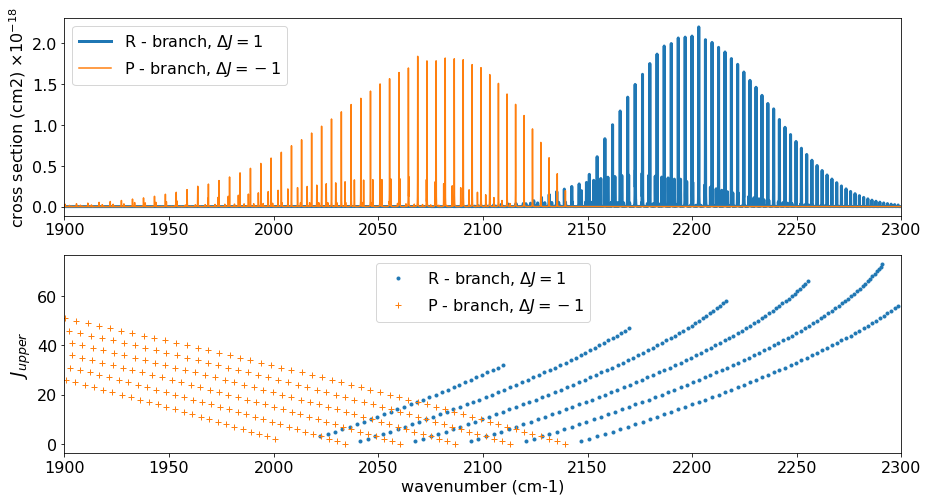
\includegraphics[width=\linewidth]{fig/branch_13_0.png}
    \caption{R-branch and P-branch cross sections in the $\Delta \nu=1$ band of carbon monoxide.}
    \label{fig:rpbranchco}
\end{figure*}

For the eigenvalue $E_r$ of the relative motion, we denote quantum states by the pair $(\nu, J)$ of vibrational quantum number $\nu$ and rotational quantum number $J$, with the initial state $(\nu,J) = (\nu_i, J_i)$ and the final state $(\nu,J) = (\nu_f, J_f)$. Consider transitions in a diatomic molecule such as carbon monoxide with $\Delta \nu = \nu_f - \nu_i = 1$ and $\Delta J = J_f - J_i = \pm 1$. Denote the eigenvalues of the relative motion for the initial and final states by $E_r = E_{r,i}$ and $E_r = E_{r,f}$, respectively, and define the transition energy $\Delta E = E_{r,f} - E_{r,i}$.

Make the coordinate transformation $q=r - r_e$. Then
\begin{align}
\label{eq:vpotent}
V_\mathrm{eff} (q) &\approx V_e + \frac{\mu}{2} \omega^2 q^2 + \frac{\hbar^2 J(J+1)}{2 \mu (q + r_e)^2} \\
&\approx V_e + \frac{\mu}{2} \omega^2 q^2 + \frac{\hbar^2 J(J+1)}{2 \mu  r_e^2},
\end{align}
so the wave equation for $\phi_r(q)$ is
\begin{align}
&- \frac{\hbar^2}{2 \mu} \frac{\partial^2}{\partial q^2} \phi_r(q) + \frac{\mu}{2} \omega^2 q^2 \phi_r(q) = E^\prime_r \phi_r(q) \\
&E^\prime = E_r - V_e - \frac{\hbar^2 J(J+1)}{2 \mu r_e^2},
\end{align}
i.e., the harmonic-oscillator wave equation. The energy eigenvalues of a harmonic oscillator with angular frequency $\omega$, with vibrational quantum number $\nu=0,1,2,\dots$, are
\begin{align}
E^\prime = \hbar \omega \left( \nu + \frac{1}{2} \right),
\end{align}
so the eigenvalues of the original wave equation are
\begin{align}
E_r = V_e + \hbar \omega \left( \nu + \frac{1}{2} \right) + \frac{\hbar^2 J(J+1)}{2 \mu r_e^2}.
\end{align}

Let
\begin{align}
E_r(\nu,J) = V_e + \hbar \omega \left( \nu + \frac{1}{2} \right) + \frac{\hbar^2 J(J+1)}{2 \mu r_e^2}.
\end{align}
Since $E_{r,f} = E(\nu_f, J_f)$ and $E_{r,i}=E(\nu_i,J_i)$, we have
\begin{align}
\Delta E &= E_{r,f} - E_{r,i} = E(\nu_f, J_f) - E(\nu_i,J_i) \\
&= \hbar (\nu_f - \nu_i) + \frac{\hbar^2}{2 \mu r_e^2} \bigl[J_f(J_f+1) - J_i(J_i+1)\bigr] \\
&= \hbar \Delta \nu + \frac{\hbar^2}{2 \mu r_e^2} (J_f-J_i)(J_f + J_i + 1) \\
\label{eq:nl}
&= \hbar \Delta \nu + \frac{\hbar^2}{2 \mu r_e^2} \Delta J \,(2 J_i + \Delta J + 1).
\end{align}

Substituting $\Delta \nu = 1$, $\Delta J = 1$ into Eq.~(\ref{eq:nl}) yields
\begin{align}
\label{eq:rbranch}
\Delta E = \hbar \omega + \frac{\hbar^2}{\mu r_e^2} (1 + J_i).
\end{align}
Substituting $\Delta \nu = 1$, $\Delta J = -1$ into Eq.~(\ref{eq:nl}) gives
\begin{align}
\label{eq:pbranch}
\Delta E = \hbar \omega - \frac{\hbar^2}{\mu r_e^2} J_i.
\end{align}

These results imply that, centered on $\hbar \omega$, the transitions form a comb with spacing $\frac{\hbar^2}{\mu r_e^2}$ to either side. Figure~\ref{fig:rpbranchco} shows the cross sections of CO for $\Delta \nu =1$, displaying this comb-like pattern. The series of lines given by Eq.~(\ref{eq:rbranch}), extending toward higher wavenumber (to the right), is the \emph{R-branch}, and that of Eq.~(\ref{eq:pbranch}) is the \emph{P-branch}.

\section{Line Profiles and Line Strengths}

Although the transition energies of molecules are discrete due to quantum-mechanical effects, the absorbed energy is broadened around those discrete energies for various reasons. This broadening is called \emph{broadening}. In planetary atmospheres, the three important types are
\begin{itemize}
    \item Doppler broadening due to thermal motion (and microturbulence),
    \item natural broadening due to the uncertainty principle,
    \item pressure broadening that depends on pressure and arises from van der Waals forces between molecules.
\end{itemize}

First, broadening due to thermal motion is caused by the Doppler shift $\nu = \hat{\nu} ( 1 + v_x/c)$ when an atom has a line-of-sight velocity $v_x$ owing to thermal motion. Because the distribution function of $v_x$ follows the Maxwell velocity distribution,
\begin{align}
P(v_x) &= \sqrt{\frac{m}{2 \pi k_B T}} \, e^{-\frac{m v_x^2}{2 k_B T}} \\
&= \sqrt{\frac{m}{2 \pi k_B T}} \, e^{-\frac{m c^2 (\nu - \hat{\nu})^2}{2 k_B T \hat{\nu}^2}},
\label{eq:dopplerveldist}
\end{align}
the line is broadened accordingly. Using the half width at half maximum (HWHM),
\begin{eqnarray}
\gamma_D = \hat{\nu} \sqrt{\frac{2 (\log{2}) k_B T}{m c^2}},
\label{eq:dopplergamma}
\end{eqnarray}
the Doppler-broadened line profile is
\begin{align}
g_D(\nu; \hat{\nu}; \gamma_D) = \sqrt{\frac{\log{2}}{\pi}} \frac{1}{\gamma_D}
\exp\!\left[ - \log{2} \left( \frac{\nu - \hat{\nu}}{\gamma_D}\right)^2 \right],
\label{eq:dopplerprofile}
\end{align}
i.e., Doppler broadening follows a Gaussian distribution. Velocity dispersion from microturbulence is likewise often approximated by a Gaussian, but is not commonly considered at present.

By contrast, pressure broadening and natural broadening are both represented by the Lorentz profile,
\begin{eqnarray}
g_L(\nu; \hat{\nu}; \gamma_L) = \frac{\gamma_L/\pi}{(\nu - \hat{\nu})^2  + \gamma_L^2},
\label{eq:lorentzprofile}
\end{eqnarray}
where $\gamma_L$ is the HWHM.

In planetary atmospheres, pressure broadening (van der Waals broadening) is especially important. For Earth’s atmosphere, one often uses the air-broadening coefficient $\gamma_{L, \mathrm{W}}^{\mathrm{air}}$, defined as $\gamma_{L, \mathrm{W}}$ at $p_0=$ 1 atmosphere and $T_0=$ 296 K, and computes
\begin{eqnarray}
\gamma_{L, \mathrm{W}}(p,T) = \gamma_{L, \mathrm{W}}^{\mathrm{air}} \frac{p}{p_0} \left( \frac{T_0}{T} \right)^\alpha,
\label{eq:airtogen}
\end{eqnarray}
where $\alpha$ is the temperature exponent (typically around 0.5, but it varies). Because pressure broadening originates from van der Waals forces exerted by surrounding molecules, it depends on the background gas composition. In particular, many exoplanet atmospheres are H$_2$/He-dominated, so values differ from those under Earth air, and care is needed.

Natural broadening is the line broadening arising from the uncertainty principle. Using the Einstein $A$ coefficient,
\begin{eqnarray}
\gamma_{L, \mathrm{n}} = \frac{A}{4 \pi c} = \frac{0.222}{4 \pi c} \left( \frac{\nu}{\mathrm{cm^{-1}}} \right)^2 \mathrm{[cm^{-1}]},
\end{eqnarray}
which reflects the excited-state survival probability $\propto e^{-A t}$ and the uncertainty relation. Unlike pressure broadening, natural broadening is more significant at low pressure.

When both the Doppler and Lorentz profiles apply, the line profile is their convolution, called the \emph{Voigt profile}\index{Voigt profile@Voigt profile}:
\begin{align}
&g_V(\nu;\hat{\nu}) = ( g_L \ast g_D )(\nu; \hat{\nu}) \nonumber \\
&= \int_{-\infty}^\infty \! d \nu^\prime \,
g_L(\nu - \nu^\prime;\hat{\nu};\gamma_L)\,
g_D(\nu^\prime - \hat{\nu};\hat{\nu};\gamma_D).
\label{eq:voigt}
\end{align}
If both pressure and natural broadening contribute, one may use
\begin{eqnarray}
\label{eq:sumgamma}
\gamma_L = \gamma_{L, \mathrm{W}} + \gamma_{L, \mathrm{n}},
\end{eqnarray}
because the convolution of two Lorentzians satisfies
\begin{align}
&g_L(\nu;\hat{\nu},\gamma_{L,\mathrm{W}}) \ast g_L(\nu;\hat{\nu},\gamma_{L,\mathrm{n}}) \nonumber \\
&= \int_\infty^\infty \! d \nu^\prime \,
g_L(\nu - \nu^\prime;\hat{\nu};\gamma_{L,\mathrm{W}})\,
g_L(\nu^\prime - \hat{\nu};\hat{\nu};\gamma_{L,\mathrm{n}}) \\
&= \frac{(\gamma_{L,\mathrm{W}}+\gamma_{L,\mathrm{n}})/\pi}{(\nu - \hat{\nu})^2  + (\gamma_{L,\mathrm{W}}+\gamma_{L,\mathrm{n}})^2} \nonumber \\
&= g_L(\nu;\hat{\nu},\gamma_{L,\mathrm{W}}+\gamma_{L,\mathrm{n}}),
\label{eq:voigt2}
\end{align}
so the HWHMs add. Note also that Lorentzian wings are not thought to extend indefinitely; beyond a certain distance from line center (on the order of $10^2\,\mathrm{cm^{-1}}$), a rapid cutoff (sub-Lorentzian behavior) is expected. Although this effect is not yet fully understood, one should take care when computing over wide wavenumber ranges.

Because line profiles are normalized as
\begin{align}
\int d \nu \, g(\nu) = 1,
\end{align}
the dimension of $g(\nu)$ is $\mathrm{cm}$.

Consider the absorption of photons by molecules. In molecular spectroscopy, it is common to express energies as wavenumbers by dividing by $hc$; we follow that convention. Since we consider absorption, the final state lies at higher energy than the initial state; we therefore relabel the final and initial states as \textit{upper} and \textit{lower}, respectively. For example, $E_\mathrm{low} = E_{\nu_i, J_i}/hc$ and $E_\mathrm{up} = E_{\nu_f, J_f}/hc$.

The strength of each absorption line is proportional to the number of molecules in the lower state $E_\mathrm{low}$, because absorption proceeds via stimulated absorption from that level. However, stimulated emission induced by the incident light reduces the effective absorption and must be included. Under local thermodynamic equilibrium,
\begin{align}
\label{eq:lte}
\frac{n_\mathrm{low}}{n} &= \frac{\mathsf{g}_\mathrm{low}}{Q(T)}
\exp\!\left(- \frac{h c E_\mathrm{low}}{k_B T} \right),
\end{align}
where $\mathsf{g}_\mathrm{low}$ is the degeneracy, $n$ is the total population, and $Q(T)$ is the partition function. The correction for stimulated emission is $(1- e^{-h c \hat{\nu}/k_B T})$, where $\hat{\nu}$ is the absorption wavenumber, i.e., the level spacing $\hat{\nu} = E_\mathrm{up} - E_\mathrm{low}$\footnote{We avoid writing this quantity directly with $E$ because, spectroscopically, the relevant observable is the wavenumber at the absorption center.}.

Including the coefficients, the \emph{line strength} is defined so that the cross section is
\begin{align}
\sigma^2 (\nu) = S(T)\, g(\nu),
\end{align}
i.e., $S(T)$ has the dimension of $\mathrm{cm}$. One obtains
\begin{align}
\label{eq:STexomol}
S(T) &= \frac{\mathsf{g}_\mathrm{up}}{Q(T)} \frac{ A}{8 \pi c \hat{\nu}^2}
e^{-  c_2 E_\mathrm{low}/T} \left(1- e^{-c_2 \tilde{\nu}/T}\right),
\end{align}
where $c_2 \equiv hc/k_B = 1.4387773 \, \mathrm{cm\,K}$ and $A$ is the Einstein $A$ coefficient.

\begin{itembox}{$\clubsuit$ Eq.~(\ref{eq:STexomol}) $\,^\dagger$}
%\tiny
\footnotesize
The effective absorption equals stimulated absorption ($B_{lu}$) minus stimulated emission ($B_{ul}$):
\begin{align}
S(T) &= \frac{h c \hat{\nu}}{c} \left( \frac{n_\mathrm{low}}{n} B_{lu} - \frac{n_\mathrm{up}}{n} B_{ul} \right).
\end{align}
Under LTE,
\begin{align}
\frac{n_\mathrm{up}}{n_\mathrm{low}} &= \frac{\mathsf{g}_\mathrm{up}}{\mathsf{g}_\mathrm{low}}
\exp\!\left(- \frac{h c (E_\mathrm{up} - E_\mathrm{low})}{k_B T} \right) \\
&= \frac{\mathsf{g}_\mathrm{up}}{\mathsf{g}_\mathrm{low}} e^{-hc \hat{\nu}/k_B T}.
\end{align}
From detailed balance,
\begin{align}
\mathsf{g}_\mathrm{low} B_{lu} &= \mathsf{g}_\mathrm{up} B_{ul}, \\
A &= 2 \pi h c \hat{\nu}^3 B_{ul}.
\end{align}
Using these,
\begin{align}
S(T) &= \frac{h \hat{\nu}}{4 \pi} \frac{n_\mathrm{low}}{n} B_{lu} \left(1 -  e^{-hc \hat{\nu}/k_B T}\right) \\
&= \frac{\mathsf{g}_\mathrm{up}}{Q(T)} \frac{ A}{8 \pi c \hat{\nu}^2}
e^{- h c E_\mathrm{low}/k_B T} \left(1- e^{- h c \tilde{\nu}/k_B T}\right),
\end{align}
where Eq.~(\ref{eq:lte}) has been used.
\end{itembox}

\section{Rovibrational Transitions of Various Molecules$^\ddagger$}

\subsection*{Methane}
%https://doi.org/10.1016/j.jqsrt.2024.108897
\begin{figure}
    \centering
    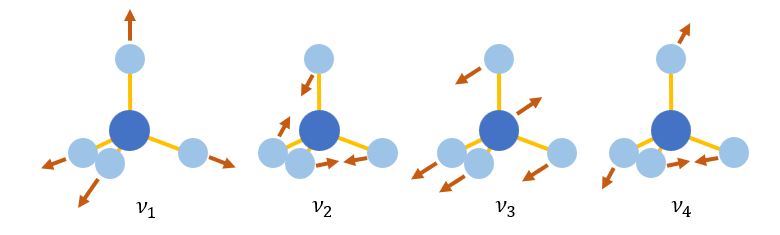
\includegraphics[width=\linewidth]{fig/methanevib.png}
    \caption{The four vibrational modes of methane.}
    \label{fig:ch4vib}
\end{figure}

As shown in Fig.~\ref{fig:ch4vib}, methane has four vibrational modes, $\nu_1, \nu_2, \nu_3,$ and $\nu_4$, of which the infrared-active modes—i.e., those that absorb photons in the infrared—are $\nu_3$ and $\nu_4$. These have strong fundamental bands at 3.25–3.45\,$\mu$m and 7.5–8.0\,$\mu$m, respectively. In addition, numerous hot bands arising from the polyad structure appear elsewhere. The polyad structure originates from the near relationships
$\nu_1 \simeq \nu_3 \simeq 2 \nu_2 \simeq 2 \nu_4 \simeq 3000\,\mathrm{cm}^{-1}$,
and is characterized by the polyad number
\begin{align}
\mathrm{P} =  2 (\nu_1 + \nu_3) + \nu_2 + \nu_4.
\end{align}
The polyads are named Monad ($P=0$), Dyad ($P=1$), Pentad ($P=2$), Octad ($P=3$), Tetradecad ($P=4$), Icosad ($P=5$), Triacontad ($P=6$), and Tetracontad ($P=7$). Their energies are roughly $1500\,P\ \mathrm{cm}^{-1}$. For example, the methane absorption seen near $1.6\,\mu$m in the $H$ band of brown dwarfs corresponds to the $P=4$ Tetradecad \cite{2024JQSRT.31608897K}.\\

\subsection*{Band Heads in Diatomic Molecules}

In the harmonic-oscillator approximation the potential is taken as a quadratic function of the internuclear separation, and in Eq.~(\ref{eq:vpotent}) the centrifugal term’s dependence on internuclear distance was ignored. In practice this approximation describes the CO $\Delta \nu=1$ transitions well (Fig.~\ref{fig:rpbranchco}). However, for larger vibrational changes $\Delta \nu$ these approximations break down as the internuclear distance changes appreciably, and a structure known as a \emph{band head} appears. The potential can be written
\begin{align}
\label{eq:vpotent_}
V_\mathrm{eff} (q) &\approx V_e + \frac{\mu}{2} \omega^2 q^2 + \frac{\hbar^2 J(J+1)}{2 \mu r_e^2 \,[1 + (q/r_e)^2]} \\
&\approx \frac{\hbar^2 J (J+1)}{2 \mu r_e^2} \left[1 - 2 \frac{q}{r_e} + 3 \left(\frac{q}{r_e} \right)^2 + \cdots \right],
\end{align}
so when $q/r_e$ becomes large the effective centrifugal term weakens. Moreover, as indicated by the ground electronic state in Fig.~\ref{fig:co_ele_state}, the potential itself departs from a quadratic form as one moves away from equilibrium. Treating these effects perturbatively (details omitted) leads to an energy expression that is quadratic in $X=(\nu + 1/2)$ and $Y=J(J+1)$. Writing a form that neglects quadratic terms other than the cross term ($XY$), we have
\begin{align}
\label{eq:nonharmo_cen}
E_r (\nu, J) &= V_e + \hbar \omega \left( \nu + \frac{1}{2} \right) + B_\nu J (J+1), \\
\label{eq:nonharmo_cen_x}
B_\nu &= \frac{\hbar^2}{2 \mu r_e^2} - \alpha_0  \left( \nu + \frac{1}{2} \right).
\end{align}
This reflects the picture that, as the vibrational amplitude increases in an anharmonic potential, the mean bond length increases and the rotational constant $B_\nu$ decreases.

From Eq.~(\ref{eq:nonharmo_cen_x}) we find $B_{\nu+1} - B_\nu = - \alpha_0$, so the R and P branches become
\begin{align}
\label{eq:u_fort_R}
h \hat{\nu}^R_{\mathrm{line}} (J_u) &= h \nu_\nu  + 2 B J_u - \alpha_0 J_u^2, \\
\label{eq:u_fort_P}
h \hat{\nu}^P_{\mathrm{line}} (J_u) &=  h \nu_\nu - 2 B (J_u + 1) - \alpha_0 (J_u + 1)^2, \\
B &\equiv B_0 + \frac{1}{2} \alpha_0,
\end{align}
i.e., quadratic functions.

If $\alpha_0 > 0$, the R-branch has a turning point at $J_u = B/\alpha_0 > 0$\footnote{By contrast, the turning point of the P-branch is at $- B/\alpha_0 < 0$, so there is no turning point in the physical region $J_l = J_u + 1 > 0$—for $\alpha_0>0$.}. Thus a maximum in wavenumber (minimum in wavelength) appears in the rovibrational transitions, and many lines cluster near this energy (lower panel of Fig.~\ref{fig:rpbranch}); this is the \emph{band head}. Figure~\ref{fig:rpbranch} shows an example of the CO band head near $2.3\,\mu$m. Note that the horizontal axis here is wavelength. When the temperature populates many levels near the band head, absorption near the band head becomes strong (upper panel of Fig.~\ref{fig:rpbranch}).

\begin{figure*}
    \centering
    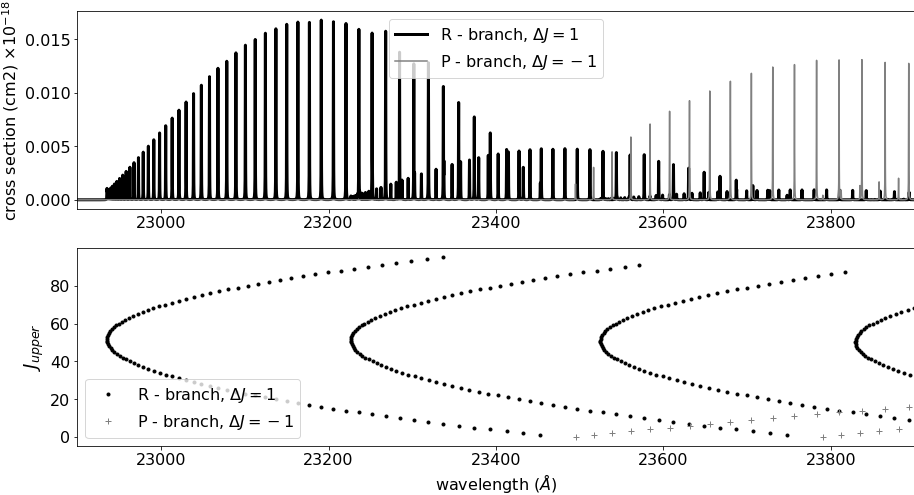
\includegraphics[width=0.9\linewidth]{fig/bandhead.png}
    \caption{Example of a band head in the CO $2.3\,\mu$m band ($X\,^1 \Sigma^+$, $\Delta \nu = 2$). Many transitions accumulate at the point where the energy of the $J_\mathrm{upper}$ levels turns over.}
    \label{fig:rpbranch}
\end{figure*}

Combining Eqs.~(\ref{eq:u_fort_R}) and (\ref{eq:u_fort_P}) into a single expression,
\begin{align}
h \hat{\nu}_{\mathrm{line}} (\mathcal{J}) &=  h \nu_\nu - 2 B \mathcal{J} - \alpha_0 \mathcal{J}^2,
\end{align}
with
\begin{align}
\mathcal{J} =
\begin{cases}
 J_u, & (\mathcal{J} > 0),\\
 - J_l, & (\mathcal{J} < 0),
\end{cases}
\end{align}
one obtains the Fortrat diagram—named after R.~Fortrat—when plotting $\mathcal{J}$ on the vertical axis against line-center wavenumber on the horizontal axis (Fig.~\ref{fig:fortrat}). There is no line at $\mathcal{J}=0$, which corresponds to the vibrational energy difference; this is called the \emph{band origin}.

\begin{figure*}
    \centering
    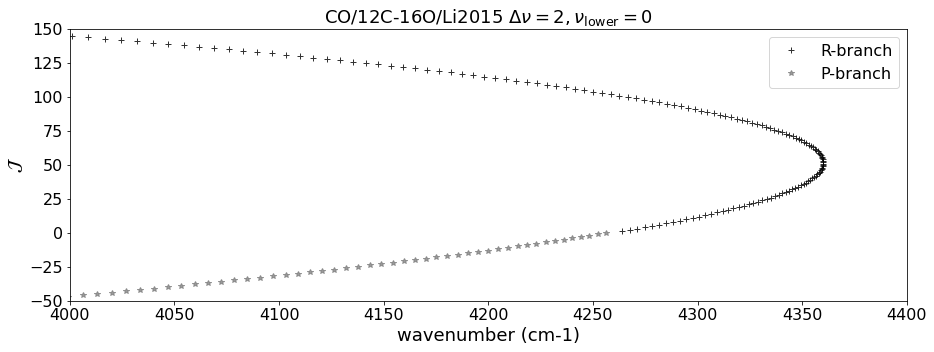
\includegraphics[width=0.9\linewidth]{fig/fortrat.png}
    \caption{Fortrat diagram for CO in the case $\Delta \nu=2$, $\nu_\mathrm{lower}=0$.}
    % exojax/documents/tutorials/Fortrat.ipynb
    \label{fig:fortrat}
\end{figure*}
